\documentclass[11pt, fleqn, a4paper, leqno]{scrartcl} %A4
\usepackage[utf8x]{inputenc} %Eingabe
\usepackage[T1]{fontenc} %Font

\usepackage[ngerman]{babel} %Trennnung
\usepackage{amsmath} %Mathesysmbole
\usepackage{graphicx} %Grafiken
\usepackage{listings} %Programmcode
\usepackage{tikz} %Grafiken malen
\usepackage{hyperref}
\hypersetup{
    colorlinks=true, %set true if you want colored links
    linktoc=all,     %set to all if you want both sections and subsections linked
    linkcolor=blue,  %choose some color if you want links to stand out
}

\definecolor{mygreen}{rgb}{0,0.6,0}
\definecolor{mygray}{rgb}{0.5,0.5,0.5}
\definecolor{mymauve}{rgb}{0.58,0,0.82}

\lstset{ %
  backgroundcolor=\color{white},   % choose the background color; you must add \usepackage{color} or \usepackage{xcolor}
  basicstyle=\footnotesize,        % the size of the fonts that are used for the code
  breakatwhitespace=false,         % sets if automatic breaks should only happen at whitespace
  breaklines=true,                 % sets automatic line breaking
  captionpos=b,                    % sets the caption-position to bottom
  commentstyle=\color{mygreen},    % comment style
  deletekeywords={...},            % if you want to delete keywords from the given language
  escapeinside={\%*}{*)},          % if you want to add LaTeX within your code
  extendedchars=true,              % lets you use non-ASCII characters; for 8-bits encodings only, does not work with UTF-8
  frame=single,                    % adds a frame around the code
  keepspaces=true,                 % keeps spaces in text, useful for keeping indentation of code (possibly needs columns=flexible)
  keywordstyle=\color{blue},       % keyword style
  language=Octave,                 % the language of the code
  morekeywords={*,...,mean,avg,clone},            % if you want to add more keywords to the set
  numbers=left,                    % where to put the line-numbers; possible values are (none, left, right)
  numbersep=5pt,                   % how far the line-numbers are from the code
  numberstyle=\tiny\color{mygray}, % the style that is used for the line-numbers
  rulecolor=\color{black},         % if not set, the frame-color may be changed on line-breaks within not-black text (e.g. comments (green here))
  showspaces=false,                % show spaces everywhere adding particular underscores; it overrides 'showstringspaces'
  showstringspaces=false,          % underline spaces within strings only
  showtabs=false,                  % show tabs within strings adding particular underscores
  stepnumber=2,                    % the step between two line-numbers. If it's 1, each line will be numbered
  stringstyle=\color{mymauve},     % string literal style
  tabsize=1,                       % sets default tabsize to 2 spaces
  title=\lstname                   % show the filename of files included with \lstinputlisting; also try caption instead of title
}


\title{Zusammenfassung: Objektorientierte Programmierung}
\author{Andreas Ruscheinski}
\date{}
\begin{document}
\maketitle
\tableofcontents
	\section{Grundbegriffe}
		\begin{description}
			\item[Kapselung:] Auf Daten können nicht direkt zugegriffen werden
			\item[Objekt:] Gegenstand des Interesses, Identität, Verhalten(Methoden), Eigenschaften[Attribute]
			\item[Attribute:] Daten einer Klasse, alle Objekte einer Klasse gleiche Eigenschaften
			\item[Methode:] Algorithmus, der einem Objekt zugeordnet ist
			\item[Botschaft:] Nachricht, die gleichnamige Methode aktiviert
			\item[Vererbung:] Weiterleitung von Informationen von oben nach unten, Unterklasse erbt Attribute, Methoden und Assoziationen oder Oberklasse
			\item[Polymorphismus:]  Eine Botschaft akiviert bei unterschiedlichen Objekten Methoden mit verschiedenen Semantiken
			\item[Dynamisches Binden:] Es wird erst zur Laufzeit entschieden, welche Methode durch eine Botschaft aktiviert wird
			\item[Konformität:] Falls Klasse A, direkt oder indirekt eine Klasse B beerbt, heißt B Nachkomme (A konform zu B)
			\item[Vorfahre:] Falls B von A erbt heisst A Vorfahre
			\item[Verfeinerung]: Geerbte Eigenschaften und Methoden werden modifiziert
			\item[Mehrfachvererbung:] Eine Klasse erbt von meheren Klassen. Problem: Vorfahren haben Methoden mit selben Name, Lösung: Umbennung
			\item[Substitutionsprinzip:] Ein Objekt einer Unterklasse kann die Rolle eines Objektes entsprechenden Oberklasse übernehmen.
			\item[Typsicheres Programm:] Es kann zur Compilezeit entschieden werden, das keine Nachricht an ein Objekt gesendet werden, für für die das Objekt keine entsprechende Schnittstelle besitzt.
			\item[Kovarianz:] Methoden einer Unterklasse sollen keine Werte zurückliefern, die man nicht Vereinbart hat
			\item[Kontravarianz:]Objekte der Oberklasse müssen durch Objekte der Unterklasse ersetzbar sein
			\end{description}
	\section{Einteilung von Patterns}
		\subsection{Anwendungsbereich: Klassenmuster}
			\begin{itemize}
				\item Beziehungen von Klassen zur Compilezeit festsetzen
			\end{itemize}
		\subsection{Anwendungsbereich: Objektmuster}
			\begin{itemize}
				\item Beziehungen zwischen Klassen beschreiben Relation von Objketen (Aggregation und Assoziation)
				\item variabel zur Laufzeit
			\end{itemize}
		\subsection{Zweck: Erzeugungsmuster}
			\begin{itemize}
				\item Aufgabe: Erzeugung von Objekten
				\item Klassenmuster: nutzen von Vererbung, zum Klasse des zu erzeugenden Objektes zu variieren
				\item Objektmuster: delegieren Objekterzeugung an ein anderes Objekt
				\item Bsp: Anzahl der erzeugten Elemente variieren oder konkrete Typ abhängig von Situation anpassen		
			\end{itemize}
		\subsection{Zweck: Strukturmuster}
			\begin{itemize}
				\item Aufgabe: Vereinfachung der Struktur zwischen Klassen
				\item Klassenmuster: nutzen Vererbung, um Schnittstellen und Implementierungen zusammenzuführen
				\item Objektmuster: Objekte zusammenzuführen
				\item Bsp: Vereinfachung von komplexen Beziehungen		
			\end{itemize}
		\subsection{Zweck: Verhaltensmuster}
			\begin{itemize}
				\item Aufgabe: Beeinflussung mit dem Verhalten von Klassen
				\item Klassenmuster: Vererbung um Verhalten unter den Klassen zu verteilen
				\item Objektmuster: Aggregation anstelle von Vererbung
				\item Bsp: Vereinfachung des Nachrichtenaustausches
			\end{itemize}
	\newpage
	\section{Software Patterns}
		\subsection{Verhaltensmuster}
		\subsubsection{Observer}
			\begin{itemize}
				\item Kategorie: Verhaltensmuster
				\item Zweck: Bei Änderungen des Zustandes sollen alle abhängigen Objekte benachrichtigt und aktualisiert werden 
				\item Akteure:
					\begin{itemize}
						\item Subjekt: kennt Liste von Beobachtern, Schnittstelle für An- und Abmelden von Beobachtern
						\item KonkretesSubjekt: speichert des Zustand und benachrichtigt alle Beobachter bei Änderungen des Zustandes
						\item Beobachter: definiert Aktualisierungsschnittstelle
						\item KonkreterBeobachter: Referenz zum KonkretenSubjekt, speichert den Zustand, implementiert Beobachter
					\end{itemize}
				\item Ablauf:
					\begin{enumerate}
						\item setState() ändert Zustand des Subjektes
						\item Änderung am Subjekt bewirkt iterative Benachrichtigung der angemeldeten Beobachter
						\item Bei Benachrichtigung des Beobachters holt dieser den neuen Zustand mit getState()
					\end{enumerate}
				\item Beispiel: Änderungen an der Börse(Konkretes Subjekt) sollen alle Broker(Konkreter Beobachter) benachrichtigt werden
			\end{itemize}
			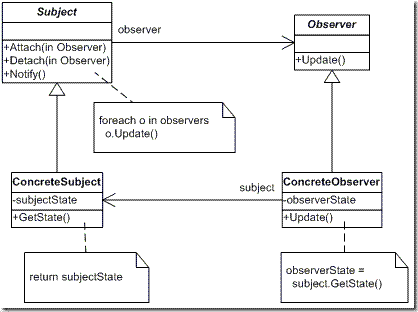
\includegraphics[scale=0.5]{images/observer.png}
		\newpage
		\subsubsection{Command}
			\begin{itemize}
				\item Kategorie: Verhaltensmuster
				\item Zweck: Für ein interaktives System soll ein Mehrstufiges, nicht limitiertes rückgängig Machen und Wiederholen von Aktionen möglich sein.
				\item Akteure: 
					\begin{itemize}
						\item Klient: erzeugt KonkreterBefehl mit Verweis zum Empfänger, gibt Aufrufer eine Referenz auf den KonkretenBefehl
						\item Empfänger: KonkreterBefehl ruft Methoden des Empfängers um seine Aktion auszuführen
						\item Aufrufer: Besitzt Verweise auf Befehle, fordert Befehle  bei Bedarf auf
						\item Befehl: definiert Schnittstelle zum Ausführen eines Befehls
						\item KonkreterBefehl: implementiert Schnittstelle, speichert Referenz zum Empfänger und für die Ausführung nötigen Zustand
					\end{itemize}
				\item Ablauf:
					\begin{enumerate}
						\item Client führt Befehl aus
						\item Befehl kennt Empfänger und ruft execute() auf Empfänger auf
						\item Implementierung von Undo und Redo über Speicherung der Befehle im Aufrufer
					\end{enumerate}
				\item Beispiel: zeilenweises Editieren mit einem Texteditor (Löschen, Ersetzen, Einfügen) und diese Aktionen rückgängig machen
			\end{itemize}
			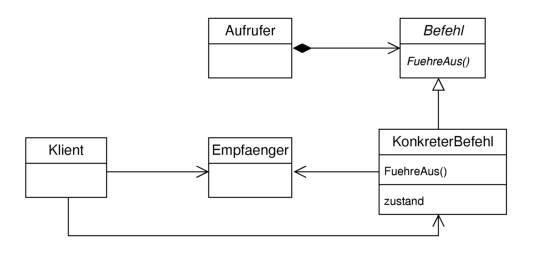
\includegraphics[scale=0.8]{images/commando.png}
			\newpage
		\subsubsection{Iterator}
			\begin{itemize}
				\item Kategorie: Verhaltensmuster
				\item Zweck: Bereitstellung einer sequentiellen Reihenfolge von zusammengesetzte Objekte (Liste, Bäume, etc) mit Abstraktion von der Datenstruktur
				\item Akteure: 
					\begin{itemize}
						\item Iterator: definiert Schnittstelle für den Besuch von Elementen
						\item KonkreterIterator: implementiert Schnittstelle für den Besuch von Elementen, achtet auf die aktuelle Position in der Datenstruktur
						\item Aggregat: definiert die Schnittstelle zur Erzeugung eines Iterators
						\item KonkretesAggregat: implementiert Schnittstelle zur Erzeugung eines Iterators
					\end{itemize}
				\item Ablauf:
					\begin{enumerate}
						\item KonrketerIterator implemtieren mit gewünschter Logik
						\item KonkretesAggregat implementierenf
						\item Arbeit mit dem Iterator
					\end{enumerate}
				\item Beispiel: Iterator über eine Liste mit Filterausdruck
			\end{itemize}
			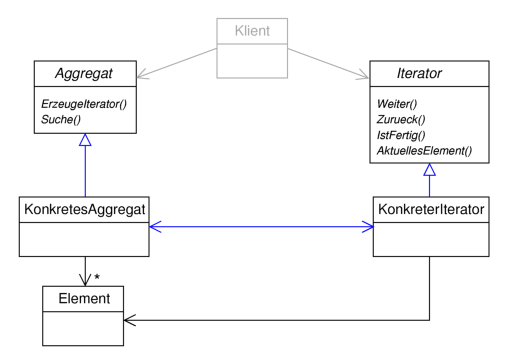
\includegraphics[scale=0.8]{images/iterator.png}
			\newpage
		\subsubsection{Mediator}
			\begin{itemize}
				\item Kategorie: Verhaltensmuster
				\item Zweck: Steuerung der Kommunikation zwischen Objekten über einen gemeinsamen Vermittler
				\item Akteure: 
					\begin{itemize}
						\item Vermittler: definiert Schnittstelle für die Kommunikation mit den Kollegen
						\item KonkreterVermittler: implementiert die Vermittler Schnittstelle für das kooperative Verhalten durch die Koordination der beteiligten Kollegen, kennt und verwaltet Kollegen-Objekte
						\item Kollegen-Klassen: jeder Kollege kennt sein Vermittler, Kommunikation mit dem Vermittler anstatt mit dem anderen Objekt Kontakt aufzunehmen
					\end{itemize}
				\item Ablauf:
					\begin{enumerate}
						\item Kollege benachrichtigt Mediator über eine Änderung
						\item Mediator benachrichtigt alle anderen Beteiligten
					\end{enumerate}
				\item Hinweis: sehr ähnlich zum Observer, Unterschied: Observer 1:n Kommunikation; Mediator: n:m Kommunikation
				\item Beispiel: Chatroom Implementierung, Kollegen sind Benutzer (Bots oder Menschen), Vermittler ist ein Zentraler Server der alle Kollegen bei Nachrichten benachrichtigt			
			\end{itemize}
			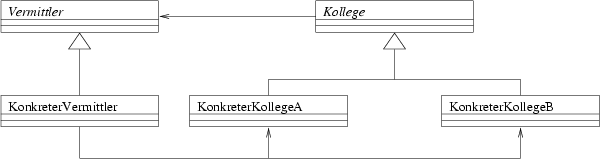
\includegraphics{images/mediator.png}
			\newpage
		\subsubsection{Visitor}
			\begin{itemize}
				\item Kategorie: Verhaltensmuster
				\item Zweck: Kapselung einer auf den Elementen einer Objektstruktur auszuführenden Operation als ein Objekt. Definition einer neuen Operation ohne Veränderung der Klasse der von ihr bearbeiteten Elemente.
				\item Akteure: 
					\begin{itemize}
						\item Besucher: deklariert Besuche-Operationen Schnittstelle für konkrete Elemente
						\item KonkreterBesucher: implementiert die Besucher Schnittstelle, jede Methode implementiert ein Fragment des Algorithmus, der auf die Struktur angewandt wird
						\item Element: Schnittstelle für NimmEntgegen-Operation
						\item KonkretesElement: implementiert Element Schnittstelle
					\end{itemize}
				\item Ablauf:
					\begin{enumerate}
						\item TODO
					\end{enumerate}
				\item Beispiel:	 TODO		
			\end{itemize}
			TODOq
			\newpage
		\subsubsection{Strategie}
			\begin{itemize}
				\item Kategorie: Verhaltensmuster
				\item Zweck: Definiert eine Familie von Algorithmen, kapselt jeden einzelnen und macht ihn austauschbar.
				\item Akteure: 
					\begin{itemize}
						\item Strategie: deklariert Schnittstelle, die von allen unterstützen Algorithmen angeboten wird
						\item KonkreteStrategie: implementiert Strategie Schnittstelle
						\item Kontext: wird mit KonkreteStrategie-Objekt konfuguriert, verwaltet die Referenz auf Strategieobjekt
						\item kann Schnittstelle definieren, die Strategieobjekten den Zugriff auf die Daten des Kontextes ermöglicht
					\end{itemize}
				\item Ablauf:
					\begin{enumerate}
						\item Strategie Schnittstelle beschreiben
						\item KonkreteStrategien implementieren
						\item Kontext mit KonkreteStrategie erstellen mit Verweis auf Strategie Schnittstelle
					\end{enumerate}
				\item Beispiel: Verschiedene Sortieralgorithmen (Strategie) für verschiedene Sortierverfahren (Quicksort, Heapsort) für eine Liste (Kontext)
			\end{itemize}
			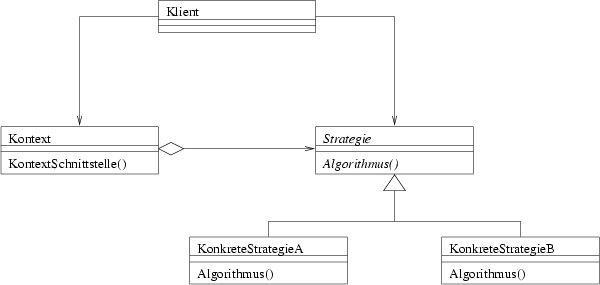
\includegraphics[scale=0.7]{images/strategie.png}
			\newpage
		\subsubsection{State}
			\begin{itemize}
				\item Kategorie: Verhaltensmuster
				\item Zweck: Ermöglicht es einen Objekt, sein Verhalten zu ändern, wenn sich sein interner Zustand geändert hat.
				\item Akteure: 
					\begin{itemize}
						\item Kontext: definiert Schnittstelle für den Klient, verwaltet eine Instanz einer konkreten Zustandsunterklasse
						\item Zustand: definiert Schnittstelle für die Kapselung des mit einem bestimmten Zustand des Kontextobjektes verbundenen Verhalten
						\item KonkreterZustand: implementiert die Zustand Schnittstelle und beschreibt das Verhalten
					\end{itemize}
				\item Ablauf:
					\begin{enumerate}
						\item Kontext definieren
						\item Zustand definieren
						\item KonkreteZustände implementieren
						\item Methodenaufruf auf Kontext ändert die Referenz auf das Zustandsobjekt durch einen neuen konkreten Zustand
					\end{enumerate}
				\item Beispiel: Eine TCPVerbindung(Kontext) ermöglicht es eine Verbindung aufzubauen, zu schließen. Die TCPVerbidung speichtert eine TCPZustand(Zustand) referenz auf einen Konkreten TCPZustand wie TCPOffen oder TCPGeschlossen
			\end{itemize}
			\newpage
		\subsection{Erzeugungsmuster}
		\subsubsection{Prototype}
			\begin{itemize}
				\item Kategorie: Erzeugungsmuster
				\item Zweck: Instanz eines Objektes wird zur Erzeugung weiterer Objekte genutzt, welche dabei Kopien der Instanz sind
				\item Akteure: 
					\begin{itemize}
						\item Prototype: Schnittstelle welche das Klonen von Objekten zusichert
						\item KonkreterPrototype: Implementiert die Schnittstelle
					\end{itemize}
				\item Ablauf:
					\begin{enumerate}
						\item Klient ruft clone() auf dem Prototype auf
						\item Klient bekommt KonkreterPrototype1 oder KonkreterPrototype2, abhängig von dem hinterlegten Prototype
					\end{enumerate}
				\item Beispiel: 
			\end{itemize}
			\begin{lstlisting}[frame=single,language=Java]
				data = getData();
				//Analyse der Daten durch verschiedene Functionen
				avgData = avg(data.clone());
				meanData = mean(data.clone());
				//data hat sich nicht veraendert
			\end{lstlisting}
			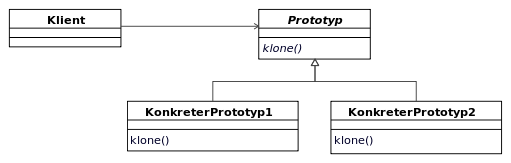
\includegraphics[scale=0.6]{images/prototype.png}
		\newpage		
		\subsubsection{Abstract Factory}
			\begin{itemize}
				\item Kategorie: Erzeugungsmuster
				\item Zweck: Bereitstellung eines Interfaces zur Erzeugung von Objekt-Familien zur Laufzeit, ohne deren konkrete Klassen festzulegen
				\item Akteure: 
					\begin{itemize}
						\item AbstrakteFabrik: definiert Schnittstelle für die Erzeugung AbstrakterProdukte einer Produktfamilie
						\item KonkreteFabrik: erzeugt KonkreteProdukte durch implementierung der AbstrakteFabrik Schnittstelle
						\item AbstraktesProdukt: definiert Schnittstelle für eine Produktart
						\item KonkretesProdukt: implementiert die AbstraktesProdukt Schnittstelle
						\item Klient: Nutzt die Schnittstelle der AbstractenFabrik und AbstrakterProdukte für weiteren Arbeitsverlauf 
					\end{itemize}
				\item Ablauf:
					\begin{enumerate}
						\item Definition der Schnittstellen
						\item Implementierung von KonkratenProdukten
						\item Implementierung von KonkretenFabriken
						\item Klient arbeitet auf den Abstrakten Schnittstellen 
					\end{enumerate}
				\item Beispiel: GUI-Programmierung, AbstraktesProdukt: Button, KonkretesProdukt: LinuxButton, WindowsButton, AbstrakteFabrik: GUI-Dialog, KonkrateFabrik: Linux-GUI-Dialog(nutzt LinuxButton) usw...
			\end{itemize}
			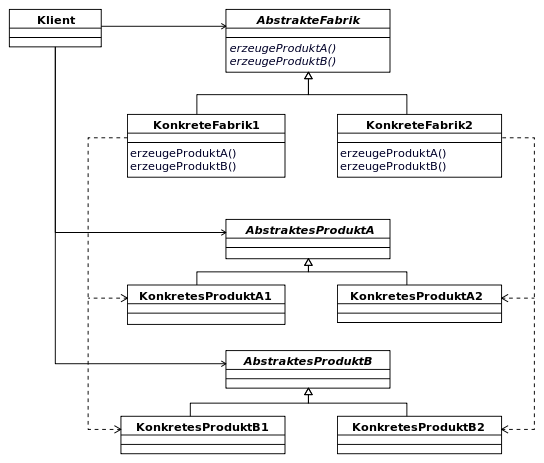
\includegraphics[scale=0.5]{images/abstract-factory.png}
			\newpage
		\subsubsection{Builder}
			\begin{itemize}
				\item Kategorie: Erzeugungsmuster
				\item Zweck: Trennung der Konstruktion komplexer Objekte von ihrer Repräsentation. Dadurch kann der gleiche Prozesss verschiedene Repräsentationen erzeugen.
				\item Akteure: 
					\begin{itemize}
						\item Erbauer: spezifiziert abstrakte Schnittstelle zur Erzeugung
						\item KonkreterErbauer: implementiert ErbauerSchnittstelle, definiert und verwaltet die von ihm erzeugte Repräsentation, ermöglicht Rückgabe von des Produktes
						\item Direktor: konstruiert ein Objekt entsprechend der Erbauerschnittstelle
						\item Produkt: repräsentiert gerade konstruierte komplexe Objekte
					\end{itemize}
				\item Ablauf:
					\begin{enumerate}
						\item Client erstellt KonkretenBuilder
						\item Client erstellt Director und weist KonkretenBuilder zu
						\item direktor.construct() bewirkt die Erstellung des Produktes
						\item builder.getResult() liefert das Produkt 
					\end{enumerate}
				\item Beispiel: Vermeidung von mehren Konstruktoren einer Klasse mit unterschiedlichen Parameter, sondern Konfiguration einer zu erstellenden Instanz über verschiedene Direktoren
			\end{itemize}
			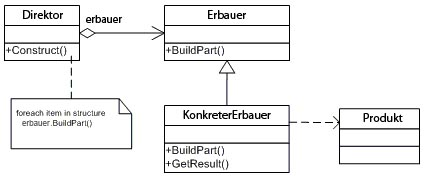
\includegraphics{images/builder.jpg}
			\newpage
		\subsubsection{Singleton}
			\begin{itemize}
				\item Kategorie: Erzeugungsmuster
				\item Zweck: Stellt sicher, dass es nur eine Instanz einer Klasse existieren kann
				\item Akteure: 
					\begin{itemize}
						\item Singleton: implementiert Logik welche garantiert das es nur eine Instance einer Klasse geben kann und bietet Schnittstelle für den Zugriff auf das Singleton Objekt
					\end{itemize}
				\item Beispiel: Erstellung einer zentralen Abstract Factory
			\end{itemize}
		\newpage
		\subsubsection{Factory Method}
			\begin{itemize}
				\item Kategorie: Erzeugungsmuster
				\item Zweck: Definiert eine Schnittstelle zur Erzeugung eines Objektes, wobei die Unterklassen entscheiden, von welcher Klasse das zu erzeugende Objekt ist.
				\item Akteure: 
					\begin{itemize}
						\item Produkt: bietet Schnittstelle nach ausssen
						\item KonkretesProdukt: implementiert die Produkt Schnittstelle
						\item Erzeuger: abstrakt, delegiert konkrete Objektinstanzierung an  Unterklasse
						\item KonkreterErzeuger: Entscheidet welches KonkretesProdukt erstellt wird
					\end{itemize}
				\item Beispiel:???
			\end{itemize}
			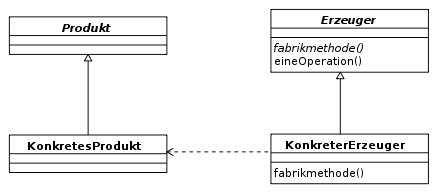
\includegraphics{images/factory-method.png}
		\newpage
		
		\subsection{Strukturmuster}
		\subsubsection{Bridge}
			\begin{itemize}
				\item Kategorie: Strukturmuster
				\item Zweck: Entkoppelung einer Abstraktion von ihrer Implementierung
				\item Akteure: 
				\begin{itemize}
					\item Abstraktion: verwaltet Referenz auf Implementierer, definiert Schnittstelle der Abstraktion
					\item SpezialisierteAbstraktion: erweitert Schnittstelle der Abstraktion
					\item Implementierer: definiert Schnittstelle für Implementierungsklassen
					\item KonkreterImplementierer: implementiert ImplementiererSchnittstelle
				\end{itemize}
				\item Ablauf:
				\begin{enumerate}
					\item Trennung der verschieden Abstraktionen von unterschiedlichen Implementierungen. Kommunikation über Brüke von Abstraktion und Implementierer
				\end{enumerate}
				\item Beispiel:			
			\end{itemize}
			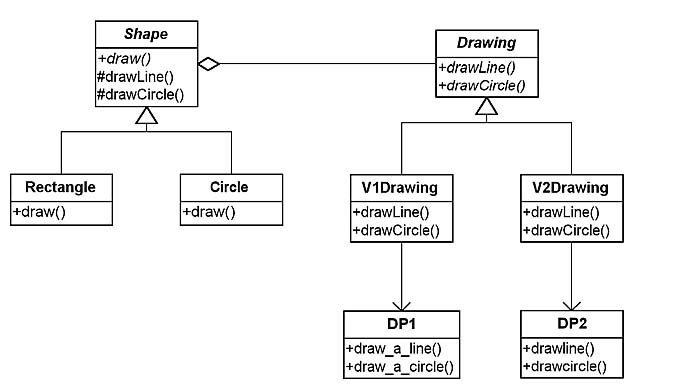
\includegraphics[scale=0.4]{images/bridge-example.jpg}\\
			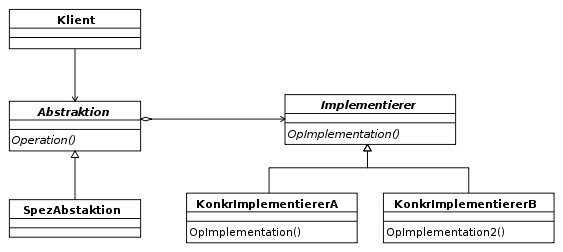
\includegraphics[scale=0.4]{images/bridge.png}
			\newpage
		\subsubsection{Adapter}
			\begin{itemize}
				\item Kategorie: Strukturmuster
				\item Zweck: Anspasssen der Schnittstellen inkompatibler Klassen
				\item Akteure: 
				\begin{itemize}
					\item Ziel: spezifiziert die neue Schnittstelle
					\item Adapter: implementiert die neue Schnittstelle und greift dabei auf Methoden der AdaptiertenKlasse zu
					\item AdaptierteKlassse: inkompatible Klasse
				\end{itemize}
				\item Ablauf:
				\begin{enumerate}
					\item Spezifikation von Ziel
					\item Implementation der Schnittstelle Ziel im Adapter unter Verwendung von Mehrfachvererbung(Klassenadapter) bzw. Objektkomposition(Objektadapter)
				\end{enumerate}
				\item Beispiel: Austausch einer Bibliothek durch eine mit ähnlichen Funktionen, dadurch viel Aufwand den Code neu anzupassen. Adapter Lösung: Altes Interface durch Nutzung der neuen Bibliothek nachstellen.
			\end{itemize}
			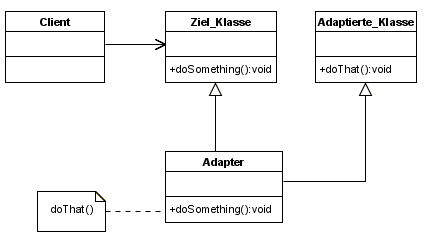
\includegraphics[scale=0.7]{images/adapter.png}
			\newpage
		\subsubsection{Proxy}
			\begin{itemize}
				\item Kategorie: Strukturmuster
				\item Zweck: Kontrolle des Zugriffes auf ein Objekt mit Hilfe eines vorgelagerten Stellvertreterobjektes
				\item Akteure: 
					\begin{itemize}
						\item Subjekt: definiert die gemeinsame Schnittstelle von Stellvertreter und realem Subjekt
						\item Proxy: implementiert die Subjekt Schnittstelle, verwaltet Referenz auf das EchteSubjekt
						\item EchtesSubjekt: das durch den Stellvertreter repräsentierte Objekt.
					\end{itemize}
				\item Beispiel: LazyLoading von Objekten aus einer Datenbank (Daten des abgerufenen Objektes werden erst angefragt wenn auf diese zugegriffen wird)
			\end{itemize}
			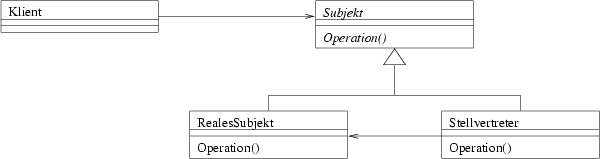
\includegraphics[scale=0.7]{images/proxy.png}
			\newpage
		\subsubsection{Composite}
			\begin{itemize}
				\item Kategorie: Strukturmuster
				\item Zweck: Zusammensetzung von Objekten zu einer Baumstruktur um eine Teil-Ganzes Hierachie. Erlaubt den Klient einzelne und zusammengesetzte Objekte einheitlich zu behandeln.
				\item Akteure: 
					\begin{itemize}
						\item Komponente: definiert als Basisklasse das gemeinsame Verhalten aller Teilnehmer.
						\item Blatt: repräsentiert Einzelobjekt, hat keine Kinder
						\item Kompositum: enthält weitere Kompositum und Blätter (dadurch entsteht die Baumstruktur)
					\end{itemize}
				\item Beispiel: Grafiken zeichnen (Komponente), eine Grafik besteht dabei aus einem Text oder Rechteck (Blatt) oder setzt sich weiter zusammen (Kompositum)
			\end{itemize}
			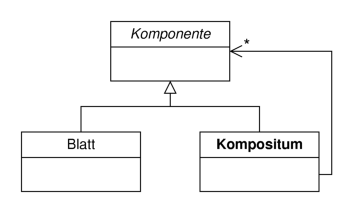
\includegraphics[scale=0.7]{images/composite.png}
			\newpage
		\subsubsection{Decorator}
			\begin{itemize}
				\item Kategorie: Strukturmuster
				\item Zweck: Erweitert ein Objekt dynamisch um Zuständigkeiten, flexible Alternative zur Unterklassenbildung, um die Funktionalität einer Klasse zu erweitern
				\item Akteure: 
					\begin{itemize}
						\item TODO
					\end{itemize}
				\item Ablauf:
					\begin{enumerate}
						\item TODO
					\end{enumerate}
				\item Beispiel: TODO
			\end{itemize}
			\newpage
		\subsubsection{Facade}
			\begin{itemize}
				\item Kategorie: Strukturmuster
				\item Zweck: Bietet eine einheitliche Schnittstelle von Schnittstellen eines Subsystems. Entkoppelt Klienten von Subystem.
				\item Akteure: 
					\begin{itemize}
						\item Facade: Implementiert eine Schnittstelle für das Subsystem welches angesprochen werden soll
					\end{itemize}
				\item Ablauf:
					\begin{enumerate}
						\item Facade implementieren so das alle benötigten Teile des Subsystemes bequem genutzt werden könne. Vorteil: Eine Facade ist zentrale Stelle für die Arbeit mit dem Subsystem, dadurch leichter zu warten und besser zum Fehler finden.
					\end{enumerate}
				\item Beispiel: Compiler(Facade) stellt Funktion zum compilieren eines Programmtextes. Das Subsystem (Parser, Scanner, Lexer, Codegenerator) werden über die Facade entsprechend der Semantik angesprochen. Man erhält also eine Kapselung der Interna eines Compilers nach außen. 
			\end{itemize}
	\section{Verhalten}

\end{document}